The next change to the structure we will test is the is the number of superdiagonals with coefficients. The initial reason for using only the first superdiagonal was to keep the preconditioner as spares as possible, to decreases the computational cost of the matrix vector product for the preconditioner. For these runs we will test with \(\left\lbrace 1,2,3,4,5\right\rbrace\) super diagonals with one partition in each, as to keep the number of coefficients low for faster learning. 

\begin{figure}[H]
    \center
    \begin{minipage}{.49\textwidth}
        \center
        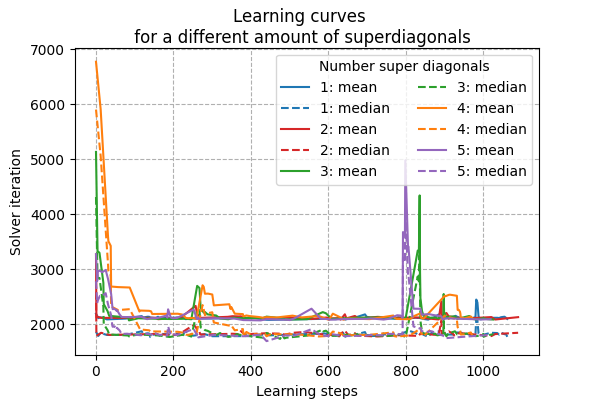
\includegraphics[width=1\textwidth]{plots/num_super_learn_curve.png}
        \caption{Learning curves for different number of superdiagonals in the preconditioner, with line style indicating mean or median solver iteration counts.\\}
        \label{fig: num super par learning curves}
    \end{minipage}    
    \begin{minipage}{.02\textwidth}
        
    \end{minipage}
    \begin{minipage}{.49\textwidth}
        \center
        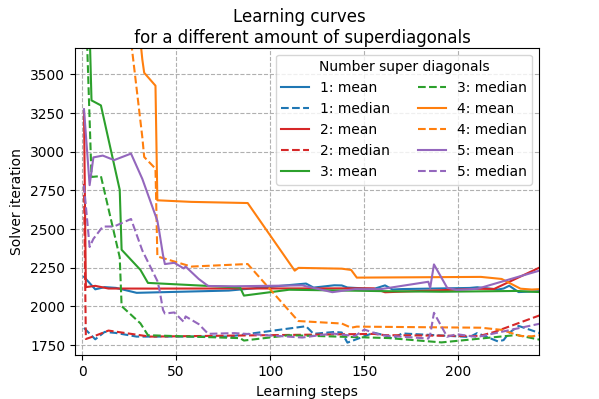
\includegraphics[width=1\textwidth]{plots/num_super_learn_curve_zoom.png}
        \caption{Learning curves for different number of super diagonals in the preconditioner, same data as figure \ref{fig: num super par learning curves} but zoomed in to the lower left corner to see the initial learning steps.}
        \label{fig: num super par learning curves zoom}
    \end{minipage}
\end{figure}

\begin{figure}[H]
    \center
    \begin{minipage}{.49\textwidth}
        \center
        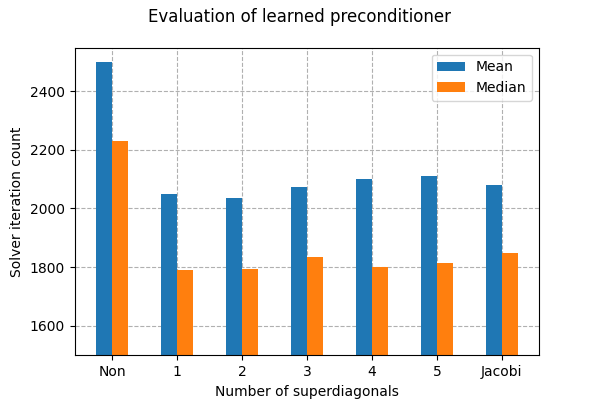
\includegraphics[width=1\textwidth]{plots/num_super_test_measure.png}
        \caption{Mean and median solver iteration count from the evaluation of the learned preconditioners with different number of super diagonals, with unpreconditioned and Jacobi preconditioned solver iteration count added for Comparison.}
        \label{fig: num super par test measure}
    \end{minipage}
    \begin{minipage}{.02\textwidth}
        
    \end{minipage}
    \begin{minipage}{.49\textwidth}
        \center
        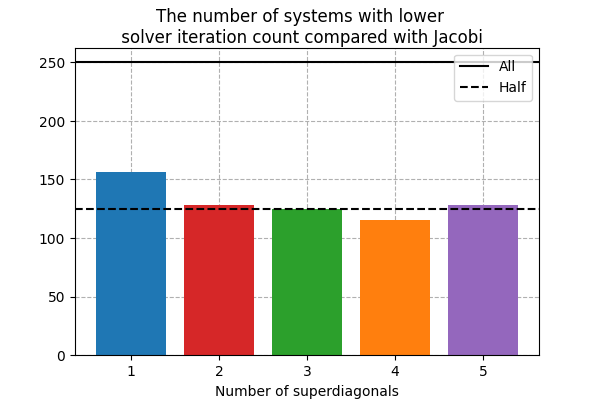
\includegraphics[width=1\textwidth]{plots/num_super_BvJ.png}
        \caption{Bar graph showing how many individual preconditioned systems have a lower solver iteration count compared to Jacobi preconditioning.\\\\}
        \label{fig: num super par BvJ}
    \end{minipage}
\end{figure}

From the learning curves, figure \ref{fig: num super par learning curves} and \ref{fig: num super par learning curves zoom}, we see similar results as the previous test, with regards to the speed of the learning and marginal differences in mean and median solver iteration counts. In the evaluation of the learned preconditioners it is as excepted with what was seen in the learning curves. Slight differences in the mean and median solver iteration counts increasing with more superdiagonals, figure \ref{fig: num super par test measure}. And in the individual iteration counts comparison, figure \ref{fig: num super par BvJ}, 1 super diagonal clearly preforms the best of the five test. Therefore we conclude that using 1 super diagonal, with no significant difference in evaluation, the faster learning, and most importantly the faster matrix vector product by having fewer nonzero entries.


% From the learning curves, figure \ref{fig: num super par learning curves} and \ref{fig: num super par learning curves zoom}, we see the similar results as the previous test, with regards to the speed of the learning, fewer coefficients leads to faster learning. There is also only a marginal differences in the learning data solver iteration counts with higher number of super diagonal being slightly worse. In the evaluation of the learned preconditioners on the testing data it is as excepted with what was seen in the learning curves. With similar conclusions, marginal differences in the mean and median solver iteration counts, figure \ref{fig: num super par test measure}, and in the individual iteration counts comparison, figure \ref{fig: num super par BvJ}, having a clear best using 1 super diagonal. Meaning it is easy conclude that using 1 super diagonal, with no significant difference in testing, the faster learning, and most importantly the faster matrix vector by the fact having fewer nonzero value.
